% Section 5.1
\section{Analysis and Discussion}\label{sec:analisis-discusion}

Our interest in identifying and classifying studies that are related to HTCondor universes that also contribute to the aforementioned academic functions was focused toward the creation and presentation of a taxonomy. Through the proposed taxonomy, we contribute to the documentary organization of these domains. See Figure~\ref{fig:taxonomia}.

This taxonomy aims to facilitate the identification and classification of HTCondor-related topics. Furthermore, it provides evidence of the domains in which the identified studies are classified, offering a structured sample that allows readers to locate those fields with the strongest relationship with the HTCondor universes.


\begin{figure}[htbp]
	\centering
	\vspace{10pt}
	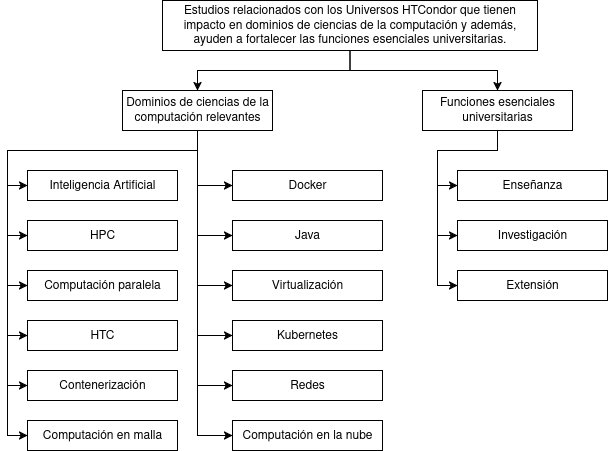
\includegraphics[scale=0.4]{resources/figures/sms-taxonomia.drawio.png}
	\vspace{6pt}
	\caption{Taxonomy of topics identified in this SMS.}
	\label{fig:taxonomia}
\end{figure}
